\section{Introduction and contributions}\label{sec:intro}
This manuscript studies how the geometry attached to a positive rational number changes when the number is moved by an explicit arithmetic map. For a reduced rational $x=a/b$ let $D(x)$ be the set of integers $d\ge2$ with $d^2\mid a$ and $d\equiv1\pmod b$; with $L=\operatorname{lcm}D(x)$ and $G=\gcd\{d-1:d\in D(x)\}$ the map is $C(x)=x+L^2/G$. We call $C$ the \emph{collective map}; it is the rational dynamics FIELD-I of the UNNS programme~\cite{FoundII}, to which the manuscript is tied by the provenance records of Appendix~\ref{app:crosswalk}. Manuscript~I of the programme~\cite{PaperI} studied the geometry that a single state carries, and Manuscript~II~\cite{PaperII} the histories of an integer generating grammar, called SELECT-II, which \cref{sec:corr} compares with $C$. The complete definition is displayed at the start of \cref{sec:notation}.

\paragraph{The question.}
Given the arithmetic state and an admissible collective transformation, \emph{which geometric changes are exactly predictable, which depend on additional relations, and which topological consequences need cellular-attachment data?} The manuscript answers this question in three layers, in the order in which the mathematics presents them: the geometry of one rational state (\cref{sec:rational,sec:relations}), the arithmetic of the dynamics and of its events (\cref{sec:regimes,sec:towers,sec:events}), and the geometry of an event, with its homology update and the towers it organises (\cref{sec:activation,sec:interval,sec:homology,sec:prediction,sec:towertop}). \Cref{sec:corr} relates the collective dynamics to SELECT-II, strictly by levels. Together with Manuscripts~I and~II it prepares a synthesis in which the three bodies of results can be compared; \emph{no universal organising law is claimed here}.

The chain of dependence just described is drawn in \cref{fig:record}.
\begin{figure}[tbp]\centering
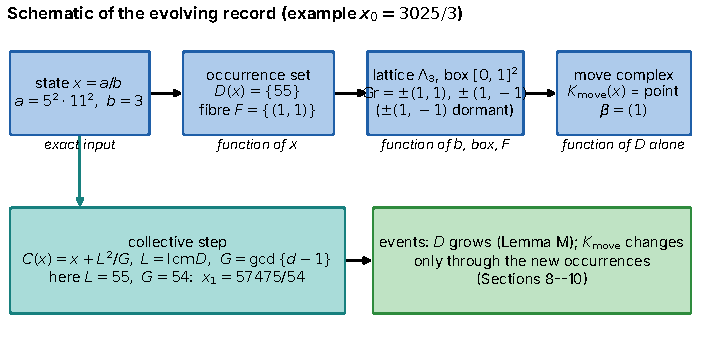
\includegraphics[width=\textwidth]{fig01_record}
\caption{\textbf{The evolving record (schematic; example values exact).} A reduced state $x=a/b$ determines its occurrence set $D(x)$ and fibre; the lattice $\Lambda_b$ and the region-Graver set depend on $b$ and the exponent box; the move complex $\Kmove$ is a function of $D$ alone (\cref{thm:R3T1a}). The collective map $C$ moves the state; the occurrence set can only grow (\cref{lem:M}); the move complex changes only through new occurrences (\cref{sec:interval}). Example $x_0=3025/3$.}\label{fig:record}
\end{figure}

\paragraph{Contributions.}
The results are organised in thirteen groups, EIII-1 to EIII-13. Each restates source records of the programme's allocation for this manuscript, which are tagged in the text by their identifiers (Appendix~\ref{app:crosswalk}).
\begin{enumerate}[leftmargin=2.7em,itemsep=2pt]
\item[\textbf{EIII-1}] \emph{Integer collapse} (\cref{sec:rational}). The complete record of an integer state is a function of its square-root content $\sigma$; the move complex is a box complex with the origin cell removed and is contractible (\cref{thm:B2T1}).
\item[\textbf{EIII-2}] \emph{Rational completeness versus relation incompleteness} (\cref{sec:rational}). For rational states the realised geometry is a function of $D(x)$ alone (\cref{thm:R3T1a}), but $D(x)$ does not determine the Graver relations: infinite families with equal $D$ and different Graver sets, for every number $k\ge2$ of primes (\cref{thm:R3T1}, uses Dirichlet's theorem), and a complete two-prime classification in seven types with one irredundant congruence bit (\cref{thm:R3T2}).
\item[\textbf{EIII-3}] \emph{Collective reduction, occurrence monotonicity, carries versus events} (\cref{sec:regimes,sec:events}). The class $G=b$ reduces to $(L,t)\mapsto(L,t+1)$ with first event at a perfect-square time (\cref{thm:R3T5a,thm:R3T5b}); $D$ is monotone along every orbit (\cref{lem:M}); arithmetic carries need not be geometric events (\cref{thm:R3T6}).
\item[\textbf{EIII-4}] \emph{Exact scaling families and a counterexample} (\cref{sec:regimes,sec:towers}). The eventual-rigidity theorem is exactly $G_\infty=1\Rightarrow$ rigid; the converse is false, with the $G=5$ tower of period $3$ and multiplier $4$ (\cref{prop:B2T7,thm:R3T5c}); the $G=11$ tower has period $8$ and multiplier $9$ (\cref{thm:R3T5bp}).
\item[\textbf{EIII-5}] \emph{The dormant-relation activation family} (\cref{sec:relations,sec:activation}). The roots $e_i-e_j$ are dormant at $x=P^2/\ell$ and realised at $y=(Pq)^2/\ell$, whose move complex is the complete graph $K_{k+1}$ with $\beta_1=\binom k2$ (\cref{thm:A4T1,thm:A4T2}).
\item[\textbf{EIII-6}] \emph{Actual dynamic activation} (\cref{sec:activation}). Reachability obstructions (a proper-divisor criterion), an eight-step orbit $3025/3\to12100/3$ with $\beta_1:0\to1$ and a $375$-step orbit with $\beta_1:0\to3$ (exact finite examples, not proofs of general reachability), and the fact that activation need not raise the Betti numbers.
\item[\textbf{EIII-7}] \emph{The exact next-event law} (\cref{sec:events}). The stage sieve $d\in D(Y_j/G)\iff Q(d)\mid Y_j$ and the resulting one-congruence-per-candidate event time; events never stop (\cref{thm:sieve,cor:event,cor:never}).
\item[\textbf{EIII-8}] \emph{Divisor-interval laws} (\cref{sec:interval}). Two occurrences are joined by an edge iff their divisor interval contains no other occurrence or $1$; when $D$ grows an old edge dies iff a new occurrence lies in its interval, and every new cell contains a new vertex (\cref{thm:A5T31,thm:A5T32}).
\item[\textbf{EIII-9}] \emph{Homology update} (\cref{sec:homology}). The zig-zag $K\leftarrow K\cap K'\to K'$ gives the identity $\Delta\beta_i=(h_i'-h_i)+(r_i'-r_i)+(r_{i-1}'-r_{i-1})$ with local $h,h'$ (\cref{thm:zigzag}) and necessary causes for any Betti change.
\item[\textbf{EIII-10}] \emph{Graph-level prediction} (\cref{sec:prediction}). Without two-cells the Betti update is predicted from the old edge set and the new occurrences alone.
\item[\textbf{EIII-11}] \emph{Event classification} (\cref{sec:prediction}). In a census of $2{,}576$ events no event is of Type~I; $1{,}787$ change the complex but no Betti number, $603$, $172$ and $14$ are of the other types (finite-exact).
\item[\textbf{EIII-12}] \emph{Nested towers} (\cref{sec:towertop}). The towers are nested filtrations without dead cells; realised moves stabilise (Graver bound $|g|_1\le\varphi(m)$); an eventual quasi-polynomial law is proved qualitatively; $G=5$ gives $(1,6,5,0)$ and $G=11$ gives $\beta_1=8$, $\beta_2=17$, $\beta_3(k+5)=\beta_3(k)+9$, all computed and verified to height $140$ and never extrapolated.
\item[\textbf{EIII-13}] \emph{Restricted correspondences and obstructions} (\cref{sec:corr}). A hierarchy of five levels of correspondence with SELECT-II, the exact classification of ratio coincidences on both towers, and the scaling obstruction: the full-period multiplier $9$ of the $G=11$ tower is not representable by any positive-length SELECT-II history.
\end{enumerate}

\paragraph{Ownership of results.}
The programme allocates to this manuscript the evolving-state, relation-lattice, occurrence-complex and collective-transformation results. A history-complex result belongs to Manuscript~II~\cite{PaperII} and a result proved in both manuscripts is proved in full in only one. Before writing, the proposed transfer was reviewed; the accepted reallocations are recorded in a derived theorem map (Appendix~\ref{app:crosswalk}) which does not alter the frozen crosswalk. In summary: the history/rewrite records B-T1--B-T9 are proved in Manuscript~II and only cited here; R3-T3, R3-T3$'$ and R3-T4 (separators and obstructions in history complexes) are cited from Manuscript~II; all other records are treated here.

\paragraph{What is not claimed.}
No physical interpretation is given. No novelty or priority claim is made. The Graver basis of the lattice is not claimed to be monotone along orbits (primitivity is not persistent; \cref{prop:A4T4b}); activation is not claimed to raise homology; tower formulas are not promoted to universal ones; finite-exact tables are never extrapolated. The programme's same-author caveat applies: all proofs and code originate from one author-collective and no independent human review is claimed. The claim C3 of the programme is not made.

\paragraph{Model boundaries.}
The collective map, the occurrence geometry and its move complexes belong to the models M5 and M8 of the programme (rational realised complexes and collective evolution). SELECT-II (M0) enters only in \cref{sec:corr}; SELECT-II is never extended to rational states. The correspondence between the integer move complex of an endpoint and the history space is cited from Manuscript~II as a non-relation (\cref{prop:A4T7}), and no map between the two dynamics is claimed (erratum ER-08).

\paragraph{Status vocabulary.}
\stat{proved} (a complete argument is given here), \stat{proved-scoped} (proved under stated hypotheses, the scope being part of the statement), \stat{finite-exact} (an exhaustive exact computation in a stated range, no claim beyond it), \stat{counterexample}, \stat{open}, \stat{cited} (taken from a released source without re-proof). \emph{Exact arithmetic} (integers and fractions, no floating point) is used in every computation; the independent engine that re-ran the finite computations of this manuscript is listed in Appendix~\ref{app:definitions}. Inherited verification suites were \emph{not re-run} (status \texttt{NOT\_RERUN}).

\paragraph{Organisation.} \Cref{sec:notation} fixes the definitions. \Cref{sec:rational,sec:relations} treat one rational state; \Cref{sec:regimes,sec:towers,sec:events} the arithmetic of the collective dynamics and of its events; \Cref{sec:activation} actual activation; \Cref{sec:interval,sec:homology,sec:prediction} the geometry of an event; \Cref{sec:towertop} the towers; \Cref{sec:corr} the correspondences; \Cref{sec:concl} the conclusions and open problems. The appendices give the source crosswalk, the definitions and engine, the complete trajectories, the relation calculations, the homology calculations and the tower tables.
